\documentclass[a4paper, 14pt]{extarticle}
\usepackage[top=1in, bottom=1in, left=1in, right=1in]{geometry}
\usepackage{amsmath}
\usepackage{amssymb}
\usepackage{graphicx}
\usepackage{fontspec}
\usepackage{hyperref}
\usepackage{tikz}
\usepackage{fontspec}
%\usetikzlibrary{decorations.pathmorphing}
\usetikzlibrary{calc,decorations,patterns,arrows,decorations.pathmorphing,positioning}
\definecolor{pltblue}{HTML}{1F77B4}
\tikzset{every picture/.style={/utils/exec={\fontspec{Pretty Neat}}}}
\setmainfont{Pretty Neat}


\makeatletter
\pgfset{
  /pgf/decoration/randomness/.initial=2,
  /pgf/decoration/wavelength/.initial=100
}
\pgfdeclaredecoration{sketch}{init}{
  \state{init}[width=0pt,next state=draw,persistent precomputation={
    \pgfmathsetmacro\pgf@lib@dec@sketch@t0
  }]{}
  \state{draw}[width=\pgfdecorationsegmentlength,
  auto corner on length=\pgfdecorationsegmentlength,
  persistent precomputation={
    \pgfmathsetmacro\pgf@lib@dec@sketch@t{mod(\pgf@lib@dec@sketch@t+pow(\pgfkeysvalueof{/pgf/decoration/randomness},rand),\pgfkeysvalueof{/pgf/decoration/wavelength})}
  }]{
    \pgfmathparse{sin(2*\pgf@lib@dec@sketch@t*pi/\pgfkeysvalueof{/pgf/decoration/wavelength} r)}
    \pgfpathlineto{\pgfqpoint{\pgfdecorationsegmentlength}{\pgfmathresult\pgfdecorationsegmentamplitude}}
  }
  \state{final}{}
}
\tikzset{xkcd/.style={decorate,decoration={sketch,segment length=0.5pt,amplitude=0.5pt}}}
\makeatother

\usepackage{etoolbox}
\AtBeginEnvironment{tabular}{\fontspec{Pretty Neat}}

\setlength{\parindent}{0pt}
\setlength{\parskip}{0.5em}
\usepackage{fancyhdr}
\usepackage{geometry}
\usepackage{adjustbox}
\usepackage{titling}
\usepackage{multicol}
\usepackage{amsmath}
\usepackage{amssymb}
\usepackage{graphicx}
\usepackage{hyperref}
\usepackage{tikz}
\usepackage{fontspec}
\usetikzlibrary{calc,decorations,patterns,arrows,decorations.pathmorphing}
\definecolor{pltblue}{HTML}{1F77B4}

\usepackage{amsmath}
\usepackage{tikz}
\usepackage{enumitem}

\title{Random Walk Characteristics Worksheet}
\author{Network Science Course}
\date{}

\begin{document}

%\maketitle
\section{Understanding Outer Products}

\begin{enumerate}
    \item Consider two vectors: $\mathbf{a} = [1, 2, 3]$ and $\mathbf{b} = [1,3,1]$. Calculate their outer product $\mathbf{a} \otimes \mathbf{b}$.

    \vspace{3cm}
    \item Without exact calculations, sketch the resulting matrix from the outer product $\mathbf{u} \otimes \mathbf{v}$ of the following pairs of vectors.
    \begin{enumerate}
        \item $\mathbf{u} = [5,4,3,2,1]$ and $\mathbf{v} = [5,4,3,2,1]$
        \item $\mathbf{u} = [1,2,4,0,0]$ and $\mathbf{v} = [3, 1, 2, 0, 0]$
        \item $\mathbf{u} = [1,1,1,-1,-1]$ and $\mathbf{v} = [1,1,1,-1,-1]$
    \end{enumerate}
    Use shading to represent the relative values in the matrix (darker shades for larger values).
    \begin{center}
    \begin{tabular}{ccc}
        (a) & (b) & (c) \\
        \begin{tabular}{|c|c|c|c|c|c|}
        \hline
        & 1 & 2 & 3 & 4 & 5 \\
        \hline
        1 & & & & & \\
        \hline
        2 & & & & & \\
        \hline
        3 & & & & & \\
        \hline
        4 & & & & & \\
        \hline
        5 & & & & & \\
        \hline
        \end{tabular}
        &
        \begin{tabular}{|c|c|c|c|c|c|}
        \hline
        & 1 & 2 & 3 & 4 & 5 \\
        \hline
        1 & & & & & \\
        \hline
        2 & & & & & \\
        \hline
        3 & & & & & \\
        \hline
        4 & & & & & \\
        \hline
        5 & & & & & \\
        \hline
        \end{tabular}
        &
        \begin{tabular}{|c|c|c|c|c|c|}
        \hline
        & 1 & 2 & 3 & 4 & 5 \\
        \hline
        1 & & & & & \\
        \hline
        2 & & & & & \\
        \hline
        3 & & & & & \\
        \hline
        4 & & & & & \\
        \hline
        5 & & & & & \\
        \hline
        \end{tabular}
    \end{tabular}
    \end{center}
\end{enumerate}

\begin{enumerate}[resume]
    \item Look at the matrices you've sketched. If these matrices represented networks, what kind of network structures might each of them represent?
\end{enumerate}

\section{Decomposing Matrices}

\begin{enumerate}[resume]
    \item Consider the following matrix representing a small network:

    \[
    \begin{bmatrix}
    3 & 2 & 1 & 0 & 1 \\
    2 & 3 & 0 & 1 & 0 \\
    1 & 0 & 3 & 2 & 1 \\
    0 & 1 & 2 & 4 & 2 \\
    1 & 0 & 1 & 2 & 3
    \end{bmatrix}
    \]

    Try to ``decompose'' this matrix into the outer product of two vectors with minimal error. Sketch the vectors and use shading to represent their values.
    \vspace{3cm}
    \item Now consider this matrix:

    \[
    \begin{bmatrix}
    8 & 4 & 2 & 1 & 0 \\
    4 & 4 & 2 & 0 & 0 \\
    2 & 2 & 2 & 1 & 0 \\
    1 & 0 & 1 & 1 & 1 \\
    0 & 0 & 0 & 1 & 1
    \end{bmatrix}
    \]

    Can you decompose this into a sum of two outer products? Sketch the vectors for each outer product and use shading.
    \vspace{3cm}
    \item For the matrix in question 7, if you had to keep only one of the two outer products, which would you choose and why? What information about the network would be preserved?
    \vspace{3cm}
\end{enumerate}

\clearpage
\section{Neural Embeddings}

\begin{enumerate}[resume]
    \item Fill in the following matrix with the number of times each pair of words co-occurs in the sentences below.

{\small
\begin{multicols}{2}
\begin{enumerate}[label=\arabic*.,itemsep=0pt,parsep=0pt]
    \item He likes hot coffee in morning
    \item She loves hot tea in night
    \item He hates cold juice in morning
    \item They dislike cold rain in night
    \columnbreak
    \item People in Paris are warm
    \item Paris has cold rain in winter
    \item My relatives in London gave me a warm welcome
    \item London has many rain in winter
\end{enumerate}
\end{multicols}
}
\begin{center}
    \begin{tabular}{l|c|c|c|c|c}
          & hot & cold & warm & rain & in \\
\hline
likes     &   &    &    &    &  \\
\hline
loves     &   &    &    &    &  \\
\hline
hates     &   &    &    &    &  \\
\hline
dislike   &   &    &    &    &  \\
\hline
Paris     &   &    &    &    &  \\
\hline
London    &   &    &    &    &  \\
\end{tabular}
\end{center}

\item Fill in these matrices with shaded cells to represent the approximate decomposition of the co-occurrence matrix (darker shades for larger values).

\begin{center}
\begin{tikzpicture}
    % First matrix - original co-occurrence matrix
    \node at (2.5,7) {Co-occurrence matrix};

    \draw (0,0) rectangle (5,6);
    \foreach \y in {1,2,3,4,5}
        \draw (0,\y) -- (5,\y);
    \foreach \x in {1,2,3,4}
        \draw (\x,0) -- (\x,6);

    % Multiplication symbol
    \node at (6,3) {$\simeq$};

    % Second matrix
    \node at (8,7) {Query matrix};
    \draw (7,0) rectangle (9,6);
    \draw (8,0) -- (8,6);
    \foreach \y in {1,2,3,4,5}
        \draw (7,\y) -- (9,\y);

    % Multiplication symbol
    \node at (10,5) {$\times$};

    % Third matrix
    \node at (13.5,7) {Key matrix};
    \draw (11,4) rectangle (16,6);
    \draw (11,5) -- (16,5);
    \foreach \x in {12,13,14,15}
        \draw (\x,4) -- (\x,6);
\end{tikzpicture}
\end{center}
\end{enumerate}

\clearpage

\begin{enumerate}[resume]
    \item In the grids below, use the first matrix to represent the words in 2D space (left), and the second matrix to represent the context of the words in 2D space (right).
    \vspace{-1cm}
    \begin{center}
    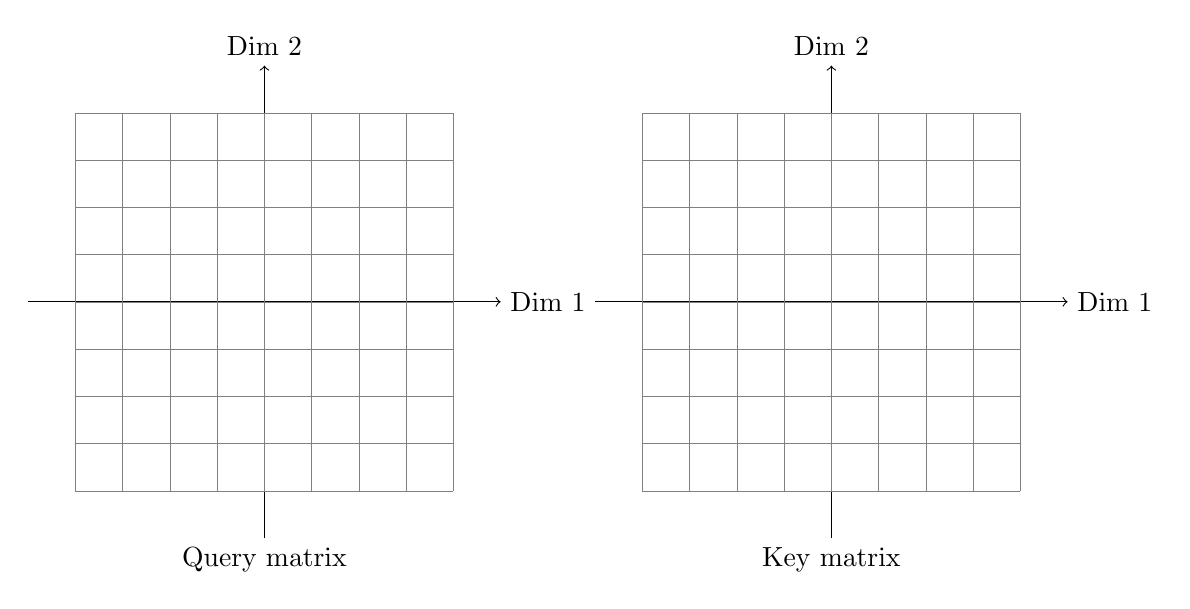
\begin{tikzpicture}[scale=0.6]
        % First grid
        \begin{scope}
            \draw[->] (-5,0) -- (5,0) node[right] {Dim 1};
            \draw[->] (0,-5) -- (0,5) node[above] {Dim 2};
            \draw[help lines] (-4,-4) grid (4,4);
            \node[below] at (0,-5) {Query matrix};
        \end{scope}

        % Second grid
        \begin{scope}[xshift=12cm]
            \draw[->] (-5,0) -- (5,0) node[right] {Dim 1};
            \draw[->] (0,-5) -- (0,5) node[above] {Dim 2};
            \draw[help lines] (-4,-4) grid (4,4);
            \node[below] at (0,-5) {Key matrix};
        \end{scope}
    \end{tikzpicture}
    \end{center}
    \vspace{-1.5em}
    \item On your 2D plot for the first matrix, mark where you would expect these new words to appear: "enjoyed", "Berlin", "dislikes". Explain your reasoning.
    \vspace{1.5cm}
    \item Sketch the matrix decomposition as a neural network. Represent the absolute value of the matrix entries by the width of the lines connecting the words and dimensions.
    \begin{center}
    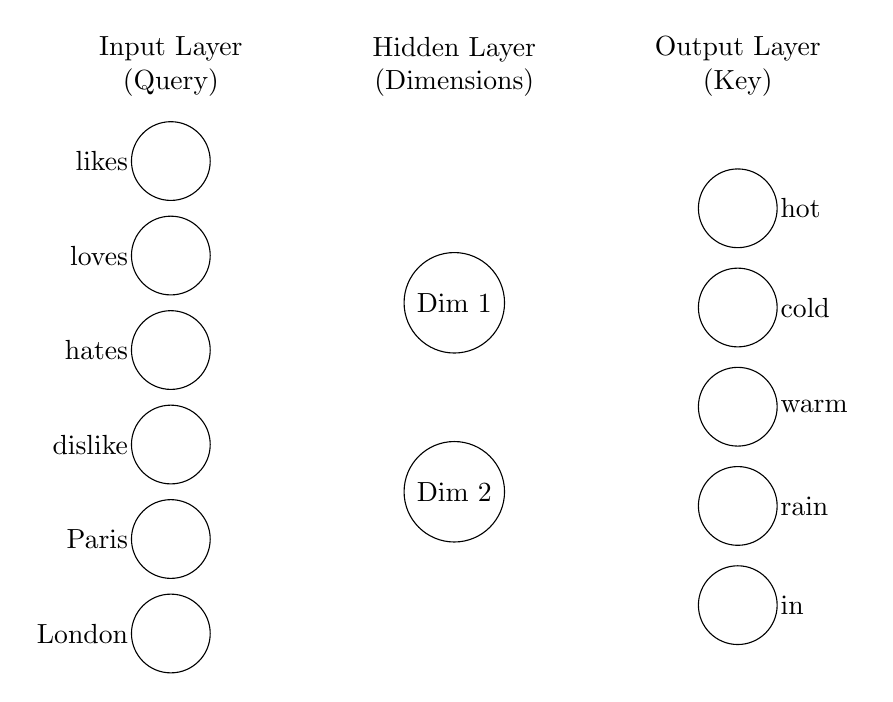
\begin{tikzpicture}[scale=0.6]
        % Input layer (words)
        \foreach \y/\word in {1/London, 2/Paris, 3/dislike, 4/hates, 5/loves, 6/likes} {
            \node[circle,draw,minimum size=1cm] (w\y) at (-2,\y*2) {};
            \node[left] at (-2.7,\y*2) {\word};
        }

        % Hidden layer (dimensions)
        \foreach \y/\dim in {1/Dim 2, 2/Dim 1} {
            \node[circle,draw,minimum size=1cm] (h\y) at (4,\y*4+1) {\dim};
        }


        % Output layer (context words)
        \foreach \y/\word in {1/in, 2/rain, 3/warm, 4/cold, 5/hot} {
            \node[circle,draw,minimum size=1cm] (o\y) at (10,\y*2.1+0.5) {};
            \node[right] at (10.7,\y*2.1+0.5) {\word};
        }

        % Label for output layer
        \node[text width=3cm, align=center] at (10,14) {Output Layer\\(Key)};

        % Labels
        \node[text width=3cm, align=center] at (-2,14) {Input Layer\\(Query)};
        \node[text width=3cm, align=center] at (4,14) {Hidden Layer\\(Dimensions)};
    \end{tikzpicture}
    \end{center}
    \vspace{0.5cm}
\end{enumerate}

\clearpage

\newpage
\subsection*{Part 4: Softmax}

Consider the word "Paris". After taking the matrix decomposition and then reconstructing the co-occurrence matrix, we get the following values for its co-occurrence with other words:
\begin{center}
\begin{tabular}{l|ccccc}
          & hot & cold & warm & rain & in \\
\hline
Paris     & -2  & 1.5  & 0.8  & 3    & -0.5
\end{tabular}
\end{center}
The following is the bar chart of these values:
\begin{center}
    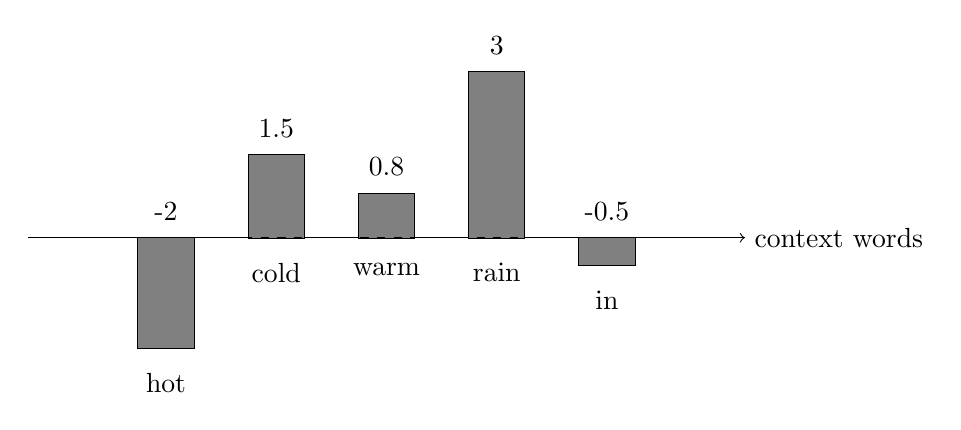
\begin{tikzpicture}[scale=0.7]
        \draw[->] (-1,-4) -- (12,-4) node[right] {context words};

        % Boxes for bars
        \draw[thick] (1,-4) rectangle (2,-6);  % hot: -2
        \draw[thick] (3,-4) rectangle (4,-2.5);  % cold: 1.5
        \draw[thick] (5,-4) rectangle (6,-3.2);  % warm: 0.8
        \draw[thick] (7,-4) rectangle (8,-1);  % rain: 3
        \draw[thick] (9,-4) rectangle (10,-4.5);  % in: -0.5

        % Bars
        \fill[gray] (1,-4) rectangle (2,-6);
        \fill[gray] (3,-4) rectangle (4,-2.5);
        \fill[gray] (5,-4) rectangle (6,-3.2);
        \fill[gray] (7,-4) rectangle (8,-1);
        \fill[gray] (9,-4) rectangle (10,-4.5);

        % Labels
        \node[below=0.2cm] at (1.5,-6) {hot};
        \node[below=0.2cm] at (3.5,-4) {cold};
        \node[below=0.2cm] at (5.5,-4) {warm};
        \node[below=0.2cm] at (7.5,-4) {rain};
        \node[below=0.2cm] at (9.5,-4.5) {in};

        % Values
        \node[above=0.1cm] at (1.5,-4) {-2};
        \node[above=0.1cm] at (3.5,-2.5) {1.5};
        \node[above=0.1cm] at (5.5,-3.2) {0.8};
        \node[above=0.1cm] at (7.5,-1) {3};
        \node[above=0.1cm] at (9.5,-4) {-0.5};

        % Zero line
        \draw[dashed] (-1,-4) -- (12,-4);
    \end{tikzpicture}
    \end{center}

\begin{enumerate}[resume]
    \item Now, imagine these values are exaggerated by taking $10$ to the power of each value. Sketch how the relative heights would change without exact calculations. Put the your estimate of the values on the y-axis for each word.
    \begin{center}
    \begin{tikzpicture}[scale=0.7]
        \draw[->] (0,0) -- (12,0) node[right] {context words};
        \draw[->] (0,0) -- (0,4) node[above] {$10^{\text{score}}$};

        % Labels
        \node[below] at (1.5,0) {hot};
        \node[below] at (3.5,0) {cold};
        \node[below] at (5.5,0) {warm};
        \node[below] at (7.5,0) {rain};
        \node[below] at (9.5,0) {in};
    \end{tikzpicture}
    \end{center}
    \item Based on your estimate, normalize these values so that they sum to 1.
\end{enumerate}


\end{document}